\documentclass{article}
\usepackage{setspace,tikz, multicol, cancel}
\usepackage[text={6.5in,8.5in},centering]{geometry}
\geometry{verbose,a4paper,tmargin=2.4cm,bmargin=2.4cm,lmargin=2.4cm,rmargin=2.4cm}
\usepackage{graphicx,amsmath,cases,multirow,appendix,graphicx,xcolor}

\usepackage{tikz}
\usetikzlibrary{trees}

\tikzset{level 1/.style={level distance=1.5cm, sibling distance=3.5cm}}
\tikzset{level 2/.style={level distance=1.5cm, sibling distance=2cm}}

\tikzset{bag/.style={text width=20em, text centered,yshift=-0.2cm}}


\setlength\parindent{0pt}

\newcommand{\note}[1]{\colorbox{gray!20}{#1}}
\newcommand*\circled[1]{\tikz[baseline=(char.base)]{
            \node[shape=circle,draw,inner sep=2pt] (char) {#1};}}

\begin{document}


\noindent\makebox[\textwidth][c]{\Large\bfseries Lecture 1 - Philosophical Principles}

\rule[0.5ex]{\linewidth}{1pt}
\textbf{Announcements}: \\
Today - Finish up class period with some philosophy of what it means to ``model'' something\\
Next class: Density-independent geometric deterministic single-species growth \\


\rule[0.5ex]{\linewidth}{1pt}

\note{Write-up on board during break}

\begin{center}

	``All models are wrong, but some are useful.''  -- Box
	
	``No model can be general, precise, and realistic.'' -- Puccia \& Levins
	
	``Make your theory as simple as possible, but no simpler.'' -- Einstein

\end{center}

\rule[0.5ex]{\linewidth}{1pt}

\section*{Categories by Type}

\begin{multicols}{2}
	[
	What is a model?\\
	Lots of categories; too many to list.\\
	Many different motivations and approaches \note{e.g., Jackson reading}\\
	$\implies$ Context for what we want to cover in course\\
	\begin{center}
	\textbf{Conceptual Models} vs. 	\textbf{Mathematical Models}
	\end{center}
	]
		\setlength{\columnseprule}{0.2pt}
	Ideas\\
	Hypotheses\\
	e.g., diagrams with boxes and arrows\\
		\begin{tikzpicture}[grow=down, -stealth, edge from parent/.style={
				draw,  <- }]
			\node[bag]{$Z$ (2$^\circ$ consumer)} 
				child{ edge from parent node[right]{$\gamma$}; 
			\node[bag]{$Y$ (1$^\circ$ consumer)}
					child{ edge from parent node[left=0.1cm]{$\alpha$}; \node[bag]{$W$}}
					child{ edge from parent node[right=0.1cm]{$\beta$}; \node[bag]{$X$}}
				};
		\end{tikzpicture}

	\columnbreak
	\begin{align*}
		Z &= \gamma Y\\
		Y &= \alpha W + \beta X
	\end{align*}
	Parameters: $\alpha$ and $\beta$\\
	State variables: $Y, W, X, Z$\\
	
\end{multicols}

\begin{center}
	\textbf{Qualitative} vs. \textbf{Quantitative}\\
	\begin{equation*}
		\Delta Z > 0 \text{ if } 
		\begin{cases}
			\Delta Y > 0 \text{ and } \gamma > 0 \\
			\Delta Y < 0 \text{ and } \gamma < 0
		\end{cases}
	\end{equation*}
	
\end{center}

\begin{multicols}{2}
	[
	\begin{center}
		\textbf{Static Models} vs. 	\textbf{Dynamical Models}
	\end{center}
	]
		\setlength{\columnseprule}{0.2pt}
	Feeding rate of $Z$ on $Y$ depends on $Y$'s abundance\\
	$\implies f(Y) = \gamma Y$
	
\begin{center}
	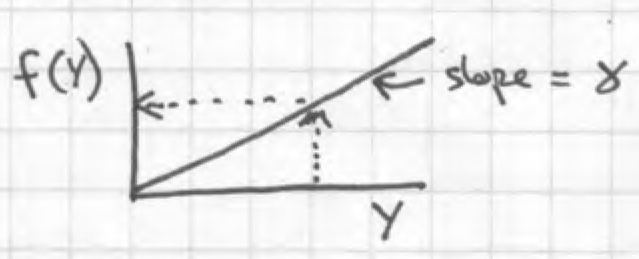
\includegraphics[width=4cm]{figs/img1}
\end{center}

	Could be non-linear
	\begin{center}
		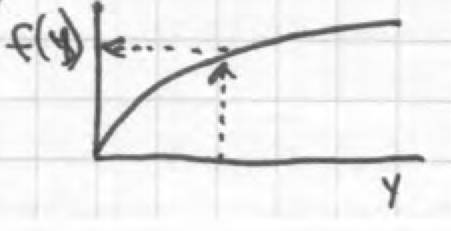
\includegraphics[width=4cm]{figs/img2}
	\end{center}
		
	\columnbreak
	
	Iterative in time or space
	\begin{equation*}
		Y_{t+1} = Y_t +( \alpha W_t + \beta X_t - \gamma Z_t  ) Y_t
	\end{equation*}
	Value of $Y$ depends on the value before it.
	
\end{multicols}

Many other types and categories: \\
\-\hspace{1cm}	Individual (agent) based\\
\-\hspace{1cm}	spatially implicit versus spatially explicit\\
\-\hspace{1cm}	etc.\\


But categories can quickly break down:\\
\-\hspace{1cm} ex1. Dynamical models contain static models\\
\-\hspace{1cm} ex2. Typically interested in \textit{qualitative} predictions from \textit{quantitative} models

\rule[0.5ex]{\linewidth}{1pt}


\section*{Categories by Purpose}
Quantitative models are tools for \textit{evaluating} hypotheses/conceptual models



\begin{multicols}{2}
	[
	Traditionally:
	\begin{center}
		\textbf{Statistical Models} vs. 	\textbf{Process Models}
	\end{center}
	]
	\setlength{\columnseprule}{0.2pt}
	Hypothesis testing \&
	Parameter estimation\\
	$\implies$ Inference within bounds of data\\
	e.g., linear regression, ANOVA, t-tests
	
	\begin{center}
	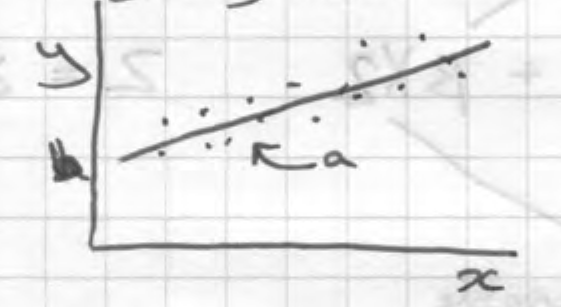
\includegraphics[width=4cm]{figs/img3}
	\begin{equation*}
		y_i = a x_i + b + \epsilon_i
	\end{equation*}

	$a$ - slope\\
	$b$ - intercept\\
	$\epsilon$ - residual errors

	$\implies$ Pattern
	
	\end{center}
	
	\columnbreak
	
	First-principals\\
	Analytical inference\\
	Simulation \& Numerical analysis\\
	
	e.g., intercept = 0 makes no sense for functional response
	\begin{center}
	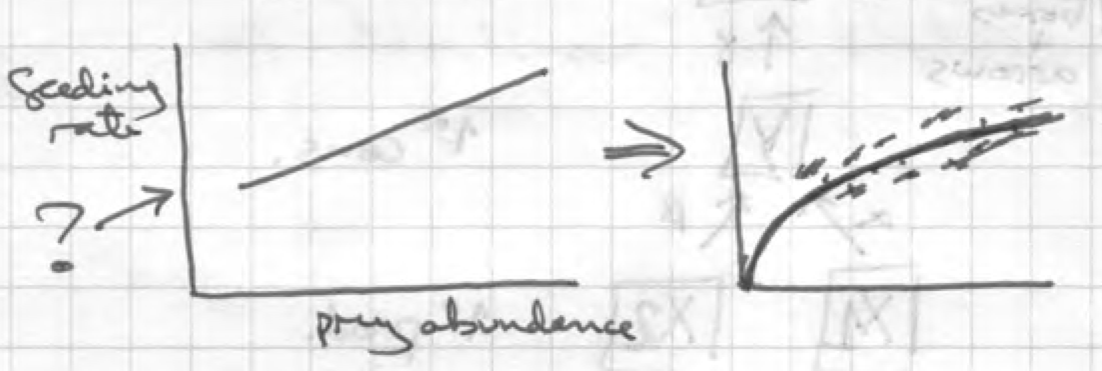
\includegraphics[width=7cm]{figs/img4}
	
	$\implies$ Mechanism
	\end{center}
\end{multicols}

The best modern-day quantitative modeling \textit{combines} traditional Statistical and Process modeling
\begin{center}
		Deterministic (mechanistic) ``core'' + Stochastic (error) shell\\
		Feeding rate = $\underbrace{f(Prey)}_{core} + \underbrace{\epsilon}_{shell}$
		\begin{equation*}
			\epsilon  \sim \mathcal{N}(0, \sigma^2)
		\end{equation*}
\end{center}

$\implies$ New world of process-model fitting \& information-theoretic model comparisons\\

Models are \textit{not} the same as hypotheses or theories\\
Multiple models can encapsulate the same hypotheses\\
Purpose is often to \textit{refine} hypotheses; a form of quantitative reasoning.\\

e.g., ``Feeding rate increases with prey abundance.'' = hypothesis

\rule[0.5ex]{\linewidth}{1pt}

\pagebreak

\section*{Model Complexity}

In Ecology: wide range of model complexities\\

\-\hspace{1cm} Discrete-time Logistic: $x_{t+1} = r x_t(1-x_t)$ \\
\-\hspace{1cm} \-\hspace{1cm}  1 parameter \& 1 state variable, yet chaotic dynamics possible!

\-\hspace{1cm} EcoPath, Atlantis (end-to-end models)\\
\-\hspace{1cm} \-\hspace{1cm} 100-1000's of parameters\\
\-\hspace{1cm} \-\hspace{1cm} 10-100's of state variables\\

We will be dealing with the former range in this class

Common criticisms of theoretical ecology:\\
\-\hspace{1cm}``Where is reality?''\\
\-\hspace{1cm}``Too simple'' ``Irrelevant''\\
\-\hspace{1cm}``Real world is way more complex than just a handful of parameters and state variables.''\\
\-\hspace{1cm}``Theory applies in general everywhere, but nowhere in particular.  Thus useless''
\\
\\
Much work has shown low-dimensional model can explain most of the observed variation.\\
Low-dimensional models allow:\\
\-\hspace{1cm}  identify \& focus on most critical parameters, variables, processes\\
\-\hspace{1cm} rigorous exploration/understanding of uncertainty\\
\-\hspace{1cm}decision-making tools\\
\-\hspace{1cm}general understanding is the goal\\

``No model can be general, precise, and realistic.'' -- Puccia \& Levins\\


\note{R demonstration: Polynomial regression - statistical model}


Have population sizes of rabbits at time $t$ -- $N(t)$\\
Model it using polynomial regression:\\
\begin{equation*}
	N(t) = \sum_{n=0}^\infty \beta_n t^n = \beta_0 \cancelto{1}{t^0} + \beta_1 t^1 + \beta_2 t^2 + \ldots + \beta_n t^n
\end{equation*}

\note{Group exercise}
Repeat with random numbers\\
What have we learned from our polynomial model?  Nothing!\\
Yet this statistical model is a perfect fit to the data!\\

$\implies$ Goal of theoretical ecology is understanding (few parameters)\\

Lotka-Volterra predator-prey model with 4 parameters:
\begin{equation*}
	\frac{dN}{dt} = N (\alpha - \beta L)  \quad  \quad
	\frac{dL}{dt}  =  L (e \beta N - d)	
\end{equation*}

[Turns out LV model is wrong for Lynx-Hare, but took a long time to realize that and provided important insights into pred-prey ecology in general.]

\rule[0.5ex]{\linewidth}{1pt}

\pagebreak

\section*{Linear vs. Nonlinear Models}
\begin{multicols}{3}
	$f(x) = \alpha + \beta x$\\
	Variable:  $x$\\
	Parameters:  $\alpha$ and $\beta$\\
	
	\columnbreak
	
	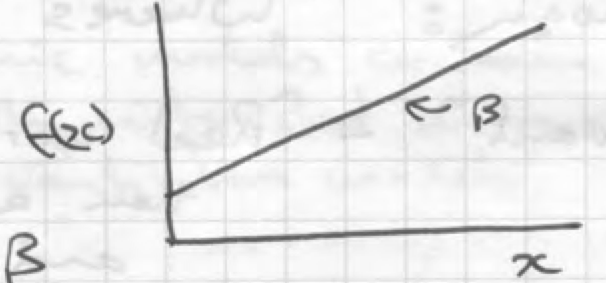
\includegraphics[width=4cm]{figs/img6}
	
	\columnbreak
	
	 $\implies$ Linear model 
\end{multicols}

\begin{multicols}{3}
	$f(x) = \alpha + \beta x^2$\\
	
	\columnbreak
	
	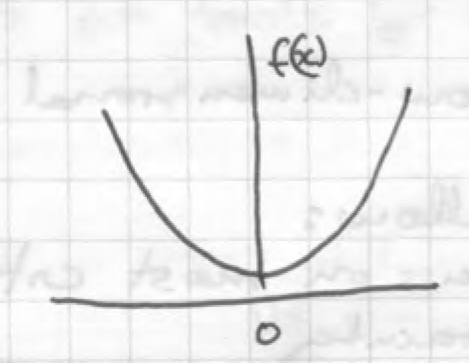
\includegraphics[width=4cm]{figs/img7}
	
	\columnbreak
	
	$\implies$ ``Nonlinear''  for ecologists \& mathematicians\\
	(nonlinear in state variable)\\
	$\implies$ ``Linear'' for statisticians\\
	(in parameters)
\end{multicols}

\begin{multicols}{3}
	$f(x) = \alpha + \beta^2 x$\\
	
	\columnbreak
	
	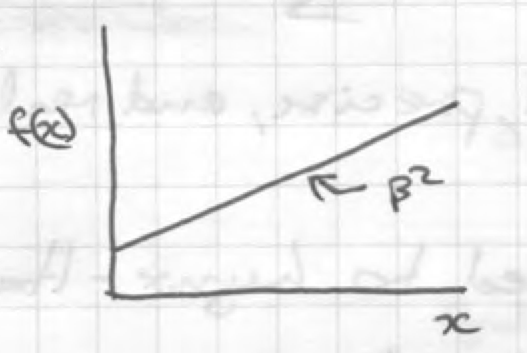
\includegraphics[width=4cm]{figs/img8}
	
	\columnbreak
	
	$\implies$ ``Linear''  for ecologists \& mathematicians\\
	$\implies$ ``Nonlinear'' for statisticians\\
	(nonlinear in parameters)
\end{multicols}

\rule[0.5ex]{\linewidth}{1pt}

\section*{My road to Theoretical Ecology}
\begin{itemize}
	\item For some, this class will be easy \& intuitive.  For others, less so.
	\item I am not a mathematician (or statistician)!  As undergrad, took usual Calculus (even remedial Calculus for biologists).  But skipping equations in papers.  Took authors on their word (esp.~discussion section).
	\item Went to grad school after 3 yrs.~as field ecologists to learn ``theoretical ecology''. (But almost failed out of first year stats class; too much calculus; over my head.)\\\\
	$\implies$ Your ability and what you learn will come down to your motivation.  Keep at it.  Persevere.
	\item My motivation: Conceptual understanding of species interaction strengths \& IGP theory.
	\item In 3rd year while reading a paper, realized I'd read and actually understood the equations!\\
	\item So much untested and interesting theory exists that is just waiting for empiricists to test \& develop \& correct
	\item Don't have to be a mathematician, but for Ecology to make progress we need to understand theory (``the math'') 
\end{itemize}

\rule[0.5ex]{\linewidth}{1pt}
\rule[0.5ex]{\linewidth}{1pt}

\end{document}